\section{Experiment 8E: control-aware private aggregation}
\label{sec:experiment8e}

\paragraph{Question.}
Experiment 8E tests whether client-level privacy noise can be redistributed
toward directions that matter less for closed-loop control, while retaining the
replacement-adjacent $(\epsilon,\delta)$ guarantee from 8C--8D. The comparison
does not change the public parameter box, cohort, privacy budget, estimator, or
controller. It changes only the public geometry in which client contributions
are clipped and Gaussian noise is calibrated.

\paragraph{Mechanism and privacy argument.}
Let $z_i\in[-1,1]^3$ be client $i$'s bounded normalized log-parameter vector and
let $W_g=\operatorname{diag}(w_g)$ be a fixed positive diagonal matrix for
public compatibility class $g$. Define
\begin{equation}
 y_i=\Pi_{C_g}(W_gz_i),\qquad C_g=\lVert w_g\rVert_2,
\end{equation}
where $\Pi_{C_g}$ is Euclidean projection onto the radius-$C_g$ ball. This ball
contains the transformed public box, since
$\lVert W_gz\rVert_2\le\lVert w_g\rVert_2$ for every
$z\in[-1,1]^3$. The release is
\begin{equation}
 \widetilde z_g=W_g^{-1}\left(\frac{1}{n}\sum_{i=1}^{n}y_i+
 \xi\right),\qquad \xi\sim\mathcal N(0,\sigma_g^2I).
\end{equation}
Under replacement adjacency, the mean in transformed coordinates has
$\ell_2$ sensitivity $2C_g/n$. Calibrating $\sigma_g$ with the same analytic
Gaussian mechanism as 8C therefore gives $(\epsilon,\delta)$ client-level DP.
Multiplication by $W_g^{-1}$, conversion to physical parameters, parameter-box
projection, and controller synthesis are deterministic post-processing and do
not weaken the guarantee. Isotropic aggregation is the special case $W_g=I$.

The family-specific weights are public and frozen before private evaluation.
They are the normalized fourth roots of central finite-difference curvatures of
mean nonlinear yaw-tracking RMSE at the public family-center plants, using the
three declared design maneuvers and a step of 0.1 in normalized log coordinates.
For example, the nominal weights are $(1.636,1.820,0.336)$. Relative to isotropic
noise, this reduces normalized standard deviations in the two tire/mass ratios
to approximately 0.87 and 0.78, while increasing that of $m/I_z$ by a factor of
4.25. This allocation is justified only if the public curvature correctly
reflects downstream control relevance; Experiment 8E tests that premise.

\paragraph{Frozen protocol and gate.}
Ten fresh training fleets, seeds 86--95, contain 100 clients per family and use
the complementary single-speed recording protocol. Separate nonlinear test
fleets contain ten clients per family. Cohorts of 10, 30, and 100 are evaluated
at $\epsilon\in\{2,4,8,\infty\}$ and $\delta=10^{-5}$ over three held-out
maneuvers. Every finite cell uses ten privacy draws. Isotropic and control-aware
runs use common standard-normal draws for a paired comparison. Fleet means,
not individual clients or privacy draws, are the independent statistical units.
The gate, fixed before execution, requires at least one finite cell to achieve
all of: at least 15\% tracking improvement over isotropic DP, at most 10\%
degradation from the common non-private mean, complete amplitude feasibility,
and worst frozen radius below one.

\begin{table}[htbp]
\centering
\caption{Experiment 8E tracking results. ``Cost'' is degradation from the
common non-private mean; ``gain'' is improvement over isotropic DP.}
\label{tab:experiment8e}
\begin{tabular}{rrrrrr}
\toprule
$n$ & $\epsilon$ & Isotropic & Control-aware & Cost & Gain\\
\midrule
10 & 2 & 0.02169 & 0.01949 & 154.22\% & 10.16\%\\
10 & 4 & 0.01523 & 0.01349 & 76.03\% & 11.39\%\\
10 & 8 & 0.01094 & 0.01005 & 31.16\% & 8.10\%\\
30 & 2 & 0.01165 & 0.01063 & 39.52\% & 8.73\%\\
30 & 4 & 0.00886 & 0.00851 & 11.74\% & 3.97\%\\
30 & 8 & 0.00810 & 0.00796 & 4.48\% & 1.73\%\\
100 & 2 & 0.00812 & 0.00797 & 4.72\% & 1.86\%\\
100 & 4 & 0.00775 & 0.00771 & 1.30\% & 0.55\%\\
100 & 8 & 0.00767 & 0.00765 & 0.52\% & 0.19\%\\
\bottomrule
\end{tabular}
\end{table}

\begin{figure}[htbp]
\centering
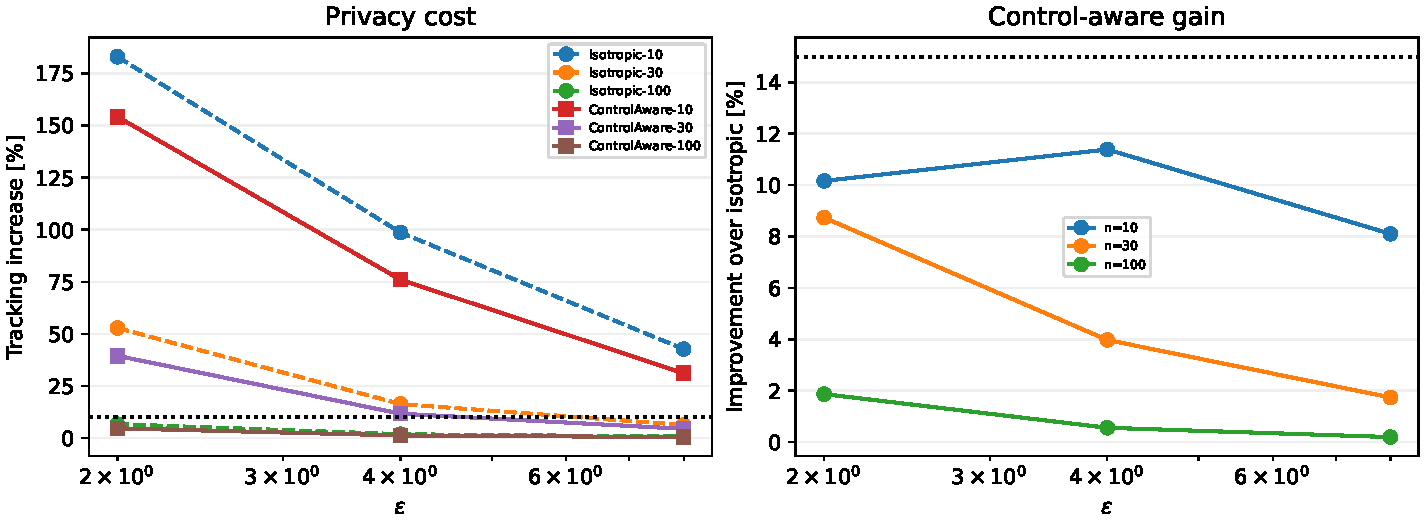
\includegraphics[width=0.9\linewidth]{../results/figures/experiment_8e_control_aware_privacy.pdf}
\caption{Privacy cost and improvement from public control-aware noise shaping.
The dashed thresholds are the frozen 10\% utility-cost and 15\% improvement
requirements.}
\label{fig:experiment8e}
\end{figure}

\paragraph{Results.}
All 3,000 local fits converge. The study retains 5,580 family releases and
167,400 client--scenario evaluations. No parameter coordinate or transformed
contribution is clipped, and every closed-loop evaluation is amplitude-feasible.
The control-aware method improves mean tracking in all nine finite cells and in
all ten independent fleets within every cell. A one-sided paired Wilcoxon test
on the ten fleet means gives $p=0.000977$ for every cell. The largest mean gain,
11.39\%, occurs for $n=10$, $\epsilon=4$; it does not reach the predeclared
15\% requirement. At the strategically important $n=30$, $\epsilon=4$ cell,
privacy cost falls from 16.36\% to 11.74\%, narrowly missing the 10\% utility
threshold. The $n=30$, $\epsilon=8$ and all $n=100$ cells satisfy the utility and
diagnostic conditions, but their improvements over isotropic DP are below 15\%.
Consequently, the joint control-aware gate fails.

\paragraph{Interpretation and decision.}
Public curvature shaping has a real and highly consistent directional effect,
but its practical magnitude is insufficient under the frozen criterion. The
benefit diminishes with cohort size because both mechanisms approach the same
non-private baseline. The result also shows why post-hoc threshold changes would
be misleading: $n=30$, $\epsilon=4$ is close to useful, yet it remains outside
the declared region. Experiment 8E must therefore be reported as a negative gate,
not as the final proposed-method validation.

The next step should not tune the diagonal weights on these private outcomes.
A defensible successor may derive a full public covariance from a stated
quadratic control-loss approximation and test it on new fleets, or retain the
simpler isotropic mechanism and focus the paper on the empirically established
cohort/privacy operating map. Partial participation and bound misspecification
remain necessary deployment tests under either choice.

\paragraph{Reproducibility.}
The frozen weights and protocol are in
\path{code/config/experiment_8e.json}; the shaped mechanism is implemented in
\path{code/src/federated_lpv/privacy.py}; and the runner is
\path{code/experiments/experiment_8e_control_aware_privacy.py}. Aggregate,
paired, and seed--draw summaries retain the complete reported evidence.
